\documentclass{standalone}
\usepackage{tikz} % Import the tikz package
\usetikzlibrary{automata} % Import library for drawing automata
\usetikzlibrary{positioning} % ...positioning nodes
\usetikzlibrary{arrows} % ...customizing arrows
\tikzset{node distance=2.5cm,
    every state/.style={
        semithick,
        fill=gray!10},
    initial text={},
    double distance=2pt,
    every edge/.style={
        draw,
        ->,>=stealth',
        auto,
        semithick}}
\let\epsilon\varepsilon
\begin{document}
    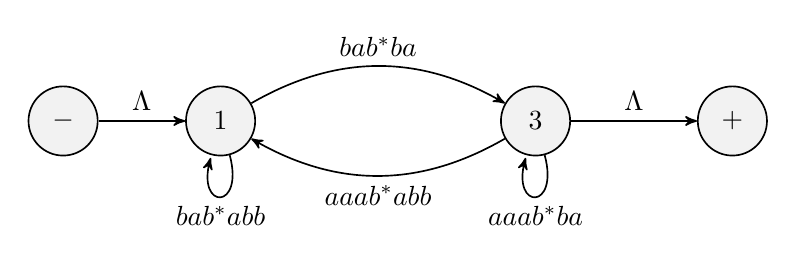
\begin{tikzpicture}
        \node[state] (start) at (0,0) {$-$};
        \node[state,] (ul) at (2,0) {$1$};

        \node[state] (ur) at (6,0) {$3$};
        \node[state,right of=ur] (end) {$+$};

        \draw (start) edge[] node {$\Lambda$} (ul); 
        \draw (ur) edge[] node {$\Lambda$} (end);
        \draw (ul) edge[bend left] node {$bab^*ba$} (ur);
        \draw (ur) edge[bend left] node {\tt $aaab^*abb$} (ul);
        \draw (ul) edge[loop below] node {$bab^*abb$} (ul);
        \draw (ur) edge[loop below] node {$aaab^*ba$} (ur);
    \end{tikzpicture}
\end{document}